\documentclass[journal,12pt,twocolumn]{IEEEtran}
%
\usepackage{setspace}
\usepackage{gensymb}
\usepackage{xcolor}
\usepackage{caption}
\usepackage[hyphens,spaces,obeyspaces]{url}
%\usepackage{subcaption}
%\doublespacing
\singlespacing

%\usepackage{graphicx}
%\usepackage{amssymb}
%\usepackage{relsize}
\usepackage[cmex10]{amsmath}
\usepackage{mathtools}
%\usepackage{amsthm}
%\interdisplaylinepenalty=2500
%\savesymbol{iint}
%\usepackage{txfonts}
%\restoresymbol{TXF}{iint}
%\usepackage{wasysym}
\usepackage{amsthm}
\usepackage{mathrsfs}
\usepackage{txfonts}
\usepackage{stfloats}
\usepackage{cite}
\usepackage{cases}
\usepackage{subfig}
%\usepackage{xtab}
%\usepackage{longtable}
\usepackage{multirow}
%\usepackage{algorithm}
%\usepackage{algpseudocode}
\usepackage{enumerate}
\usepackage{mathtools}
%\usepackage{eenrc}
%\usepackage[framemethod=tikz]{mdframed}
\usepackage[breaklinks]{hyperref}
%\usepackage{breakcites}
\usepackage{listings}
\usepackage[latin1]{inputenc}                                 %%
\usepackage{color}                                            %%
\usepackage{array}                                            %%
\usepackage{longtable}                                        %%
\usepackage{calc}                                             %%
\usepackage{multirow}                                         %%
\usepackage{hhline}                                           %%
\usepackage{ifthen}                                           %%
%optionally (for landscape tables embedded in another document): %%
\usepackage{lscape}     

\usepackage{tikz}
\usepackage{circuitikz}
\usepackage{karnaugh-map}
\usepackage{pgf}
\usepackage[hyphenbreaks]{breakurl}
\usepackage{makecell}

%\usepackage{url}
%\def\UrlBreaks{\do\/\do-}





%\usepackage{stmaryrd}


%\usepackage{wasysym}
%\newcounter{MYtempeqncnt}
\DeclareMathOperator*{\Res}{Res}
%\renewcommand{\baselinestretch}{2}
\renewcommand\thesection{\arabic{section}}
\renewcommand\thesubsection{\thesection.\arabic{subsection}}
\renewcommand\thesubsubsection{\thesubsection.\arabic{subsubsection}}

\renewcommand\thesectiondis{\arabic{section}}
\renewcommand\thesubsectiondis{\thesectiondis.\arabic{subsection}}
\renewcommand\thesubsubsectiondis{\thesubsectiondis.\arabic{subsubsection}}

% correct bad hyphenation here
\hyphenation{op-tical net-works semi-conduc-tor}

%\lstset{
	%language=C,
	%frame=single, 
	%breaklines=true
	%}

%\lstset{
	%%basicstyle=\small\ttfamily\bfseries,
	%%numberstyle=\small\ttfamily,
	%language=Octave,
	%backgroundcolor=\color{white},
	%%frame=single,
	%%keywordstyle=\bfseries,
	%%breaklines=true,
	%%showstringspaces=false,
	%%xleftmargin=-10mm,
	%%aboveskip=-1mm,
	%%belowskip=0mm
	%}

%\surroundwithmdframed[width=\columnwidth]{lstlisting}
\def\inputGnumericTable{}                                 %%
\lstset{
	%language=C,
	frame=single, 
	breaklines=true,
	columns=fullflexible
}
\graphicspath{ {./title/} } 

\begin{document}
	%
	
	\theoremstyle{definition}
	\newtheorem{theorem}{Theorem}[section]
	\newtheorem{problem}{Problem}
	\newtheorem{proposition}{Proposition}[section]
	\newtheorem{lemma}{Lemma}[section]
	\newtheorem{corollary}[theorem]{Corollary}
	\newtheorem{example}{Example}[section]
	\newtheorem{definition}{Definition}[section]
	%\newtheorem{algorithm}{Algorithm}[section]
	%\newtheorem{cor}{Corollary}
	\newcommand{\BEQA}{\begin{eqnarray}}
		\newcommand{\EEQA}{\end{eqnarray}}
	\newcommand{\define}{\stackrel{\triangle}{=}}
	
	\bibliographystyle{IEEEtran}
	%\bibliographystyle{ieeetr}
	
	\providecommand{\nCr}[2]{\,^{#1}C_{#2}} % nCr
	\providecommand{\nPr}[2]{\,^{#1}P_{#2}} % nPr
	\providecommand{\mbf}{\mathbf}
	\providecommand{\pr}[1]{\ensuremath{\Pr\left(#1\right)}}
	\providecommand{\qfunc}[1]{\ensuremath{Q\left(#1\right)}}
	\providecommand{\sbrak}[1]{\ensuremath{{}\left[#1\right]}}
	\providecommand{\lsbrak}[1]{\ensuremath{{}\left[#1\right.}}
	\providecommand{\rsbrak}[1]{\ensuremath{{}\left.#1\right]}}
	\providecommand{\brak}[1]{\ensuremath{\left(#1\right)}}
	\providecommand{\lbrak}[1]{\ensuremath{\left(#1\right.}}
	\providecommand{\rbrak}[1]{\ensuremath{\left.#1\right)}}
	\providecommand{\cbrak}[1]{\ensuremath{\left\{#1\right\}}}
	\providecommand{\lcbrak}[1]{\ensuremath{\left\{#1\right.}}
	\providecommand{\rcbrak}[1]{\ensuremath{\left.#1\right\}}}
	\providecommand{\ceil}[1]{\left \lceil #1 \right \rceil }
	\theoremstyle{remark}
	\newtheorem{rem}{Remark}
	\newcommand{\sgn}{\mathop{\mathrm{sgn}}}
	\providecommand{\abs}[1]{\left\vert#1\right\vert}
	\providecommand{\res}[1]{\Res\displaylimits_{#1}} 
	\providecommand{\norm}[1]{\lVert#1\rVert}
	\providecommand{\mtx}[1]{\mathbf{#1}}
	\providecommand{\mean}[1]{E\left[ #1 \right]}
	\providecommand{\fourier}{\overset{\mathcal{F}}{ \rightleftharpoons}}
	%\providecommand{\hilbert}{\overset{\mathcal{H}}{ \rightleftharpoons}}
	\providecommand{\system}{\overset{\mathcal{H}}{ \longleftrightarrow}}
	%\newcommand{\solution}[2]{\textbf{Solution:}{#1}}
	\newcommand{\solution}{\noindent \textbf{Solution: }}
	\providecommand{\dec}[2]{\ensuremath{\overset{#1}{\underset{#2}{\gtrless}}}}
	%\numberwithin{equation}{subsection}
	\numberwithin{equation}{section}
	%\numberwithin{problem}{subsection}
	%\numberwithin{definition}{subsection}
	\makeatletter
	\@addtoreset{figure}{problem}
	\makeatother
	
	\let\StandardTheFigure\thefigure
	%\renewcommand{\thefigure}{\theproblem.\arabic{figure}}
	\renewcommand{\thefigure}{\theproblem}
	
	
	%\numberwithin{figure}{subsection}
	
	%\numberwithin{equation}{subsection}
	%\numberwithin{equation}{section}
	%%\numberwithin{equation}{problem}
	%%\numberwithin{problem}{subsection}
	\numberwithin{problem}{section}
	%%\numberwithin{definition}{subsection}
	%\makeatletter
	%\@addtoreset{figure}{problem}
	%\makeatother
	\makeatletter
	\@addtoreset{table}{problem}
	\makeatother
	
	\let\StandardTheFigure\thefigure
	\let\StandardTheTable\thetable
	%%\renewcommand{\thefigure}{\theproblem.\arabic{figure}}
	%\renewcommand{\thefigure}{\theproblem}
	\renewcommand{\thetable}{\theproblem}
	%%\numberwithin{figure}{section}
	
	%%\numberwithin{figure}{subsection}
	
	\vspace{3cm}
	\title{
		
		\centering
		JK Flip flops Implementation using D flip flops (Synchronous Counter)
		\centering
		
	}

	
	
	% paper title
	% can use linebreaks \\ within to get better formatting as desired
	%\title{Matrix Analysis through Octave}
	%
	%
	% author names and IEEE memberships
	% note positions of commas and nonbreaking spaces ( ~ ) LaTeX will not break
	% a structure at a ~ so this keeps an author's name from being broken across
	% two lines.
	% use \thanks{} to gain access to the first footnote area
	% a separate \thanks must be used for each paragraph as LaTeX2e's \thanks
	% was not built to handle multiple paragraphs
	%
	
	\author{Satheesh K Simhachalam$^{*}$% <-this % stops a space
		\thanks{*The author is a PhD scholar with the Department
			of Electrical Engineering, Indian Institute of Technology, Hyderabad
			502285 India e-mail:  ee22resch11010@iith.ac.in. All content in this manual is released under GNU GPL.  Free and open source.}% <-this % stops a space
		%\thanks{J. Doe and J. Doe are with Anonymous University.}% <-this % stops a space
		%\thanks{Manuscript received April 19, 2005; revised January 11, 2007.}}
}
% note the % following the last \IEEEmembership and also \thanks - 
% these prevent an unwanted space from occurring between the last author name
% and the end of the author line. i.e., if you had this:
% 
% \author{....lastname \thanks{...} \thanks{...} }
%                     ^------------^------------^----Do not want these spaces!
%
% a space would be appended to the last name and could cause every name on that
% line to be shifted left slightly. This is one of those "LaTeX things". For
% instance, "\textbf{A} \textbf{B}" will typeset as "A B" not "AB". To get
% "AB" then you have to do: "\textbf{A}\textbf{B}"
% \thanks is no different in this regard, so shield the last } of each \thanks
% that ends a line with a % and do not let a space in before the next \thanks.
% Spaces after \IEEEmembership other than the last one are OK (and needed) as
% you are supposed to have spaces between the names. For what it is worth,
% this is a minor point as most people would not even notice if the said evil
% space somehow managed to creep in.



% The paper headers
%\markboth{Journal of \LaTeX\ Class Files,~Vol.~6, No.~1, January~2007}%
%{Shell \MakeLowercase{\textit{et al.}}: Bare Demo of IEEEtran.cls for Journals}
% The only time the second header will appear is for the odd numbered pages
% after the title page when using the twoside option.
% 
% *** Note that you probably will NOT want to include the author's ***
% *** name in the headers of peer review papers.                   ***
% You can use \ifCLASSOPTIONpeerreview for conditional compilation here if
% you desire.




% If you want to put a publisher's ID mark on the page you can do it like
% this:
%\IEEEpubid{0000--0000/00\$00.00~\copyright~2007 IEEE}
% Remember, if you use this you must call \IEEEpubidadjcol in the second
% column for its text to clear the IEEEpubid mark.



% make the title area
\maketitle

\tableofcontents

\bigskip

\renewcommand{\thefigure}{\theenumi}
\renewcommand{\thetable}{\theenumi}

\begin{abstract}
%\boldmath
This manual explains steps to implement JK flip flop synchronous counters with D flip flops using finite state machine.
\end{abstract}

\setcounter{figure}{0}
\setcounter{table}{0}

\section{\textbf{The Assignment}}
\begin{enumerate}[1.]
\item \textbf{Problem Statement:} A synchronus counter using two J-K flip flops that goes through the sequence of states: Q\textsubscript{1}Q\textsubscript{2} = $00 \rightarrow 10 \rightarrow 01 \rightarrow 11 \rightarrow 00$ .. is required as mentioned in Fig. \ref{fig:JKcounter}.  We need to implement this sequencing logic in ide, assembly and avr-gcc using D-flip flops. The {\em state transitioning } decoder and {\em display} decoder are part of {\em combinational} logic, while the {\em delay} is part of {\em sequential} logic.

\begin{figure}[!h]
	\begin{center}
	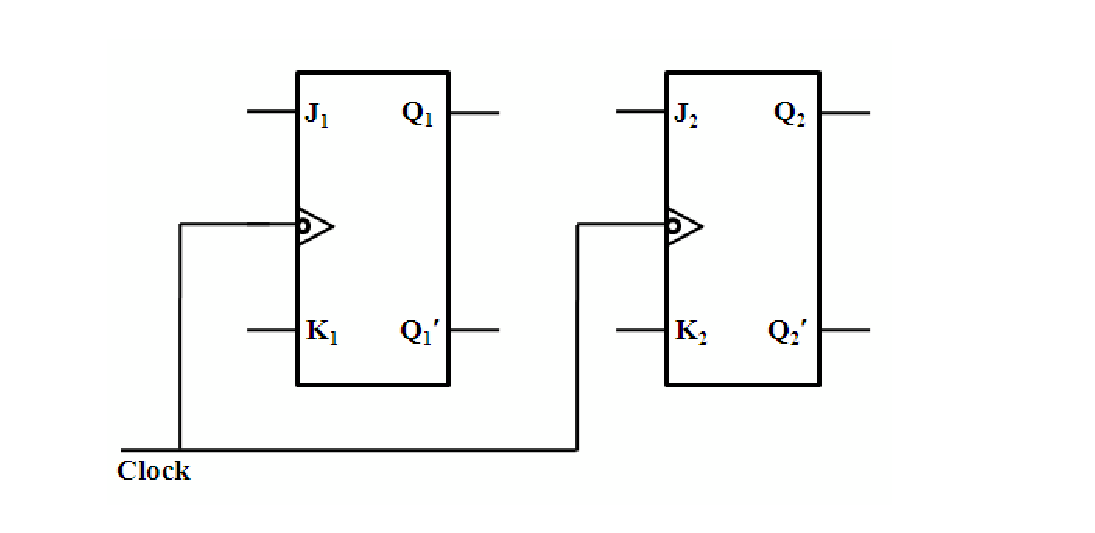
\includegraphics[width=7cm,height=4cm]{./JK1}
\end{center}
\caption{Synchronous counter with JK flip flops}
\label{fig:JKcounter}
\end{figure}
%

\item The required J and K inputs for 2 J-K flip flops are as mentioned in the Table \ref{table:JK_table}. \\

\begin{table}[h!] 
	\begin{center}
		\begin{tabular}{ |c|c|c|c|c|c|c|c| } 
			\hline
			\multicolumn{2}{|c|}{Present state} &\multicolumn{2}{|c|}{Next state} & \multicolumn{4}{|c|}{Flip flop Inputs}  \\
			\hline
			\thead{X \\ (Q\textsubscript{1})} & \thead{W \\(Q\textsubscript{2})} & \thead{B \\(Q\textsubscript{1}\textsuperscript{+})} & \thead{A \\ (Q\textsubscript{2}\textsuperscript{+})} & J\textsubscript{1} & K\textsubscript{1} & J\textsubscript{2} & K\textsubscript{2}  \\ 
			\hline
			0 & 0 & 1 & 0 & 1 & X & 0 & X  \\ 
			\hline
			1 & 0 & 0 & 1 & X & 1 & 1 & X  \\ 
			\hline
			0 & 1 & 1 & 1 & 1 & X & X & 0  \\ 
			\hline
			1 & 1 & 0 & 0 & X & 1 & X & 1  \\
			\hline
		\end{tabular}
		\caption{JK flip flop State Transition Table}
		\label{table:JK_table}
	\end{center}
\end{table}

\item From the columns of J\textsubscript{1},K\textsubscript{1}, J\textsubscript{2},K\textsubscript{2}, \\
we can say \\
\begin{equation} \label{eq:1}
	J\textsubscript{1} = 1
\end{equation}
\begin{equation} \label{eq:2}
	K\textsubscript{1} = 1 
\end{equation}
\begin{equation} \label{eq:3}
	J\textsubscript{2} = Q\textsubscript{1}
\end{equation}
\begin{equation} \label{eq:4}
	K\textsubscript{2} = Q\textsubscript{1}
\end{equation}
%
\end{enumerate}
\section{\textbf{Realization of JK flip flop using D flip flop}}
%
\begin{enumerate}[1.]

 

\item Now, we have to design to realize JK flip flop using a D flip flop. D flip flop is primarily meant to provide delay as the output of this flip flop is same as the input. \\

The first thing that needs to be done for this conversion is to draw the truth table for both the flip flops as shown in Table \ref{table:JKD_table}. The next step is to create the equivalent K-Maps for the required outputs. \\

\begin{table}[h!]
	\begin{center}
		\begin{tabular}{ |c|c|c|c|c| } 
			\hline
	J & K & Q & $Q^{+}$ & D \\
			\hline
			0 & 0 & 0 & 0 & 0 \\ 
			\hline
			0 & 0 & 1 & 1 & 1 \\ 
			\hline
			0 & 1 & 0 & 0 & 0 \\ 
			\hline
			0 & 1 & 1 & 0 & 0 \\
			\hline
			1 & 0 & 0 & 1 & 1 \\
			\hline
			1 & 0 & 1 &1 & 1 \\
			\hline
			1 & 1 & 0 & 1 & 1 \\
			\hline
			1 & 1 & 1 & 0 & 0 \\
			\hline
		\end{tabular}
		\caption{JK vs D Transition Table}
		\label{table:JKD_table}
	\end{center}
\end{table}

\item The K-Map for required input- output relation is as shown in Fig \ref{fig:kmap_a}

\begin{figure}[!h]
	\resizebox {\columnwidth} {!} {
		\begin{karnaugh-map}[4][2][1][][]
    \maxterms{0,2,3,7}
    \minterms{1,4,5,6}
    \implicantedge{1}{1}{5}{5}
    \implicantedge{4}{4}{6}{6}
    % note: posistion for start of \draw is (0, Y) where Y is
    % the Y size(number of cells high) in this case Y=2
    \draw[color=black, ultra thin] (0, 2) --
    node [pos=0.7, above right, anchor=south west] {$KQ$} % Y label
    node [pos=0.7, below left, anchor=north east] {$J$} % X label
    ++(135:1);
        
    \end{karnaugh-map}

	}
	\caption{K-map for $D$.}
	\label{fig:kmap_a}
\end{figure}

\item Obtain the state transition equations for \textbf{D} from Fig. \ref{fig:kmap_a}
\begin{equation} \label{eq:5}
	D = JQ^{\prime}+K^{\prime}Q
\end{equation}

\end{enumerate}

\section{\textbf{Finite State Machine}}
\begin{enumerate}[1.]

\item Fig. \ref{fig:fsm_counter} shows a {\em finite state machine} (FSM) diagram for the counter in Fig. \ref{fig:JKcounter}.    

\begin{figure}[!h]
	\centering
	\resizebox {\columnwidth} {!} {
		\usetikzlibrary{arrows,automata, positioning, calc}
%\usetikzlibrary{arrows,automata, calc}
%\begin{tikzpicture}[->,shorten >=1pt,node distance=2cm,on grid,auto] 
\begin{tikzpicture}[->,auto] 
   \node[ ] (s_00)   {}; 
 %  \foreach \i [count=\ni from 1] in {90,180,...,270}
%       \node[state] (s_\ni) [above right = {2*sin(\i)} and {2*(cos(\i)} of s_00]  {\ni};
        \node[state] (s_2) [above right = {2*sin(90)} and {2*(cos(90)} of s_00]  {$s_2$};        
        
         \node[state] (s_1) [above right = {2*sin(180)} and {2*(cos(180)} of s_00]  {$s_1$}; 
         \node[state] (s_3) [above right = {2*sin(270)} and {2*(cos(270)} of s_00]  {$s_3$}; 
                 
        \node[state,initial] (s_0) [above right = {0} and {2} of s_00]  {$s_0$};     

% \foreach \i  [count=\j from 1] in {0,1,...,2}
		\path	(s_0) edge [bend right]  (s_2) ;
        \path	(s_2) edge [bend right]  (s_1) ;
        \path	(s_1) edge [bend right]  (s_3) ;
		\path	(s_3) edge [bend right]  (s_0) ;		
           
\end{tikzpicture}

		}
	\caption{FSM for the counter}
	\label{fig:fsm_counter}
\end{figure}

\item From \ref{eq:5}, D inputs for D flip flops are derived using the following equations

\begin{equation}
	Q\textsubscript{1}\textsuperscript{+} = D\textsubscript{1} = J\textsubscript{1}Q\textsubscript{1}^{\prime}+K\textsubscript{1}^{\prime}Q\textsubscript{1}	
\end{equation}
Substituting values for J\textsubscript{1}, K\textsubscript{1} from \ref{eq:1} and \ref{eq:2}, 
\begin{equation}
	Q\textsubscript{1}\textsuperscript{+} = D\textsubscript{1} = 1Q\textsubscript{1}^{\prime}+0Q\textsubscript{1}	
\end{equation}
\begin{equation}
	Q\textsubscript{1}\textsuperscript{+} = D\textsubscript{1} = Q\textsubscript{1}^{\prime} 
\end{equation}
Similarly, 
\begin{equation}
	Q\textsubscript{2}\textsuperscript{+} = D\textsubscript{2} = J\textsubscript{2}Q\textsubscript{2}^{\prime}+K\textsubscript{2}^{\prime}Q\textsubscript{2}	
\end{equation}
Substituting values for J\textsubscript{2}, K\textsubscript{2} from \ref{eq:3} and \ref{eq:4},
\begin{equation}
	Q\textsubscript{2}\textsuperscript{+} = D\textsubscript{2} = Q\textsubscript{1}Q\textsubscript{2}^{\prime}+Q\textsubscript{1}^{\prime}Q\textsubscript{2}	
\end{equation}
\begin{equation}
	Q\textsubscript{2}\textsuperscript{+} = D\textsubscript{2} = Q\textsubscript{1}Q\textsubscript{2}^{\prime}+Q\textsubscript{1}^{\prime}Q\textsubscript{2}
\end{equation}

\item The {\em state transition table} for the FSM is Table \ref{table:counter_decoder} where the present state is denoted by the variables $W(Q\textsubscript{2}),X(Q\textsubscript{1})$ and the next state by $A(Q\textsubscript{2}\textsuperscript{+}),B(Q\textsubscript{1}\textsuperscript{+})$. 

\begin{table}[h!]
	\begin{center}
		\begin{tabular}{ |c|c|c|c| } 
			\hline
	X & W & B & A \\
			\hline
			0 & 0 & 1 & 0  \\ 
			\hline
			1 & 0 & 0 & 1  \\ 
			\hline
			0 & 1 & 1 & 1  \\ 
			\hline
			1 & 1 & 0 & 0 \\
			\hline
		\end{tabular}
		\caption{State Transition Table for D flip flops}
		\label{table:counter_decoder}
	\end{center}
\end{table}

The associated equations are:

\begin{equation}
	A = XW^{\prime}+WX^{\prime}
\end{equation}

\begin{equation}
	B = X^{\prime}
\end{equation}

\end{enumerate}

\section{\textbf{Implementation Details}}
\begin{enumerate}[1.]

\item Connect the Arduino, 7447, 7474 as per the details mentioned in Table \ref{table:Connection_table} and Fig \ref{fig:dec_counter}

\item The code for IDE implementation is avaialble at the following github link

\begin{lstlisting}
https://github.com/satheeshsimha/fwc-2/blob/main/ide/assignment/codes/assignment1D_ide.cpp
\end{lstlisting}

\item The code for  assembly implementation is avaialble at the following github link
\begin{lstlisting}

https://github.com/satheeshsimha/fwc-2/blob/main/assembly/assignment/codes/assignment1.asm
\end{lstlisting}

\item The code for  avr-gcc implementation is avaialble at the following github link
\begin{lstlisting}
https://github.com/satheeshsimha/fwc-2/blob/main/avr-gcc/assignment/codes/main.c
\end{lstlisting}

\vspace{2cm}

\begin{table}[h!]
	\begin{center}
		\begin{tabular}{ |c|c|c|c|c|c|c|c|c|c|c|c|c|c| } 
			\hline
			\multicolumn{1}{|c|}{} &\multicolumn{2}{|c|}{\textbf{INPUT}} & \multicolumn{2}{|c|}{\textbf{OUTPUT}} &\multicolumn{2}{|c|}{\textbf{CLOCK}} &\multicolumn{4}{|c|}{\textbf{5V}} &\multicolumn{3}{|c|}{\textbf{GND}}\\
			\hline
			\multicolumn{1}{|c|}{} & \multicolumn{1}{|c|}{W} & \multicolumn{1}{|c|}{X} & \multicolumn{1}{|c|}{A} & \multicolumn{1}{|c|}{B} & \multicolumn{2}{|c|}{} & \multicolumn{4}{|c|}{} & \multicolumn{3}{|c|}{}   \\
			\hline
			\multicolumn{1}{|c|}{Arduino} & \multicolumn{1}{|c|}{D8} & \multicolumn{1}{|c|}{D9} & \multicolumn{1}{|c|}{D2} & \multicolumn{1}{|c|}{D3} & \multicolumn{2}{|c|}{D13} & \multicolumn{4}{|c|}{} & \multicolumn{3}{|c|}{}\\
			\hline
			\multicolumn{1}{|c|}{7474} & \multicolumn{1}{|c|}{5} & \multicolumn{1}{|c|}{9} & \multicolumn{1}{|c|}{2} & \multicolumn{1}{|c|}{12} & \multicolumn{1}{|c|}{CLK1} & \multicolumn{1}{|c|}{CLK2} & \multicolumn{1}{|c|}{1} & \multicolumn{1}{|c|}{4} & \multicolumn{1}{|c|}{10} & \multicolumn{1}{|c|}{13} & \multicolumn{3}{|c|}{7} \\
			\hline
			\multicolumn{1}{|c|}{7447} & \multicolumn{2}{|c|}{} & \multicolumn{1}{|c|}{7} & \multicolumn{1}{|c|}{1} & \multicolumn{2}{|c|}{} & \multicolumn{4}{|c|}{16} & \multicolumn{1}{|c|}{8} & \multicolumn{1}{|c|}{2} & \multicolumn{1}{|c|}{6}\\
			\hline
		\end{tabular}
		\caption{Connection Diagram}
		\label{table:Connection_table}
	\end{center}
\end{table}

\begin{figure}[!h]
%	\begin{center}
%	\includegraphics[width=7cm,height=10cm]{./decade}
\resizebox {\columnwidth} {!} {
  %\documentclass{article}

%\usepackage[latin1]{inputenc}
%\usepackage{tikz}
%\usetikzlibrary{shapes,arrows}

%%%%<
%\usepackage{verbatim}
%\usepackage[active,tightpage]{preview}
%\PreviewEnvironment{tikzpicture}
%\setlength\PreviewBorder{5pt}%
%%%%>

%\begin{comment}
%:Title: Simple flow chart
%:Tags: Diagrams

%With PGF/TikZ you can draw flow charts with relative ease. This flow chart from [1]_
%outlines an algorithm for identifying the parameters of an autonomous underwater vehicle model. 

%Note that relative node
%placement has been used to avoid placing nodes explicitly. This feature was
%introduced in PGF/TikZ >= 1.09.

%.. [1] Bossley, K.; Brown, M. & Harris, C. Neurofuzzy identification of an autonomous underwater vehicle `International Journal of Systems Science`, 1999, 30, 901-913 


%\end{comment}


%\begin{document}
%\pagestyle{empty}


% Define block styles
\tikzstyle{decision} = [diamond, draw, fill=blue!20, 
    text width=4.5em, text badly centered, node distance=3cm, inner sep=0pt]
%\tikzstyle{block} = [rectangle, draw, fill=blue!20, 
%    text width=5em, text centered, rounded corners, minimum height=4em]
\tikzstyle{block} = [rectangle, draw, 
    text width=5em, text centered, rounded corners, minimum height=4em]

\tikzstyle{line} = [draw, -latex']
\tikzstyle{cloud} = [draw, ellipse,fill=red!20, node distance=3cm,
    minimum height=2em]
    
\begin{tikzpicture}[node distance = 3cm, auto]
    % Place nodes
    \node [block] (init) {Sequential Counter};
%    \node [cloud, left of=init] (expert) {expert};
%    \node [cloud, right of=init] (system) {system};
    \node [block, below of=init, node distance = 4cm] (identify) {Display Decoder};
    \node [block, below of=identify ] (evaluate) {Seven-Segment Display};
%    \node [block, right of=identify, node distance = 4cm] (delay) {Delay};
     %\node [block, (4,-3)] (q1) {Delay};
	\node at (4,-2)[block] (delay) {Delay};
\begin{scope}[->,>=latex]
    \foreach \i in {3,1}
    { 
%      \draw[->] ([yshift=\i * 0.2 cm]identify.east) -- ([yshift=\i * 0.2 cm]delay.west) ;
      \draw[->] ([xshift=\i * 0.2 cm]delay.north) |- ([yshift=\i * 0.2 cm]init.east) ;
      \draw[->] ([xshift=\i * 0.2 cm]init.south) -- ([xshift=\i * 0.2 cm]identify.north) ;
       \draw node at (\i * 0.2,-2+\i * 0.2) { \textbullet} ;
       \draw[->] (\i * 0.2,-2+\i * 0.2) -- ([yshift=\i * 0.2 cm]delay.west) ;
      
    }
\foreach \i in {-3,...,3}
    { 
      \draw[->] ([xshift=\i * 0.35 cm]identify.south) -- ([xshift=\i * 0.35 cm]evaluate.north) ;
    }
\foreach [count=\i] \j in {a,b,...,g}{
            \node (\i) at ( 1.6-\i * 0.35, -5.5) {\j} ;
            }
\foreach [count=\i] \j in {A,B}{
            \node (\i) at ( 0.8-\i * 0.4, -1.0-\i*0.4) {\j} ;
            }

\foreach [count=\i] \j in {W,X}{
            \node (\i) at ( 1.6, 1.2-\i*0.4) {\j} ;
            }
    
\end{scope}

 %   \node [block, left of=evaluate, node distance=3cm] (update) {update model};
  %  \node [decision, below of=evaluate] (decide) {is best candidate better?};
%    \node [block, below of=decide, node distance=3cm] (stop) {stop};
    % Draw edges
%    \path [line] (init) -- (identify);
  %  \path [line] (identify) -- (evaluate);
%    \path [line] (evaluate) -- (decide);
  %  \path [line] (decide) -| node [near start] {yes} (update);
   % \path [line] (update) |- (identify);
 %   \path [line] (decide) -- node {no}(stop);
%    \path [line,dashed] (expert) -- (init);
%    \path [line,dashed] (system) -- (init);
%    \path [line,dashed] (system) |- (evaluate);
\end{tikzpicture}
%}

%\end{document}

}
%\end{center}

\caption{The Synchronous counter with LED Display}
\label{fig:dec_counter}
\end{figure}




\end{enumerate}



	
	
%\begin{figure}[!h]
	
%	\centering
%	\resizebox {\columnwidth} {!} {
%		\input{./figs/fsm_down1}
%	}
%	\caption{FSM for the decade counter.}
%	\label{fig:fsm_down}
%\end{figure}
\bibliography{IEEEabrv,gvv_kmap_fsm}
\end{document}


